\section{Kontextabgrenzungen}
\subsection{Kontext Diagramm}

\begin{figure}
    \centering
    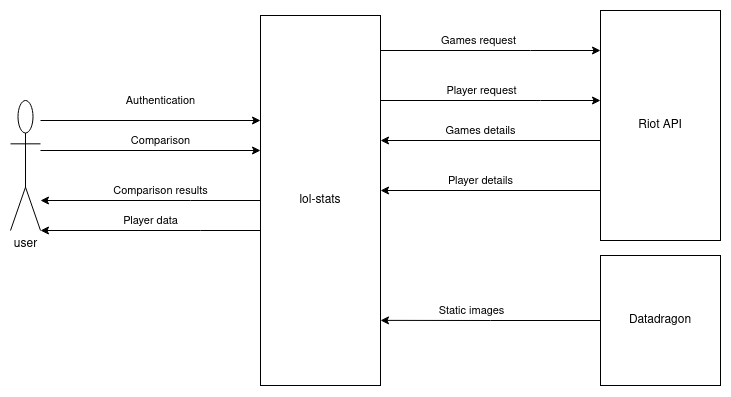
\includegraphics[width=\textwidth]{images/03-context-diagram}
    \caption{Context Diagramm der Applikation}
    \label{fig:context-diagram}
\end{figure}

In Abbildung~\ref{fig:context-diagram} ist das Context Diagramm der Applikation zu sehen.
Der User kann über eine Webseite mit der Applikation kommunizieren.
Ein User kann sich authentifizieren und danach Spieldaten anschauen.
Außerdem kann er sich mit anderen Spielern vergleichen.

Um an die Spiele und Spieler zu kommen, werden Anfragen an die Riot API gestellt.
Zusätzlich zur Riot API, die dynamische Daten zur Verfügung stellt, werden statische Assets über die Datadragon
Webseite geladen.
Diese Webseite wird von Riot für diesen Zweck zur Verfügung gestellt.

\subsection{Riot API}\label{riot-api-libraries}
Die Riot API ist eine Schnittstelle, mit mehreren Endpoints. Für dieses Projekt sind nur Endpoints des Spiels League of Legends interessant. Genauer werden die folgenden Endpoints verwendet:
\begin{itemize}
\item \textbf{League-V4:} Erlaubt mittels der SummonerID den Rang eines Spieler abzufragen
\item \textbf{Match-V5:} Hier können alle MatchIDs eines Spieler erhalten werden, mit welchen dann wiederum genaue Informationen zu den einzelnen Matches requested werden können
\item \textbf{Summoner-V4:} Hier können Informationen zu einem Spieler abgefragt werden (wie z.B. SummonerID, Name, Level, ...)
\end{itemize}
Alle diese Anfragen können einfach per HTTP an die API geschickt werden. Die API jedoch Antwort dann verschiedene Fehler-Codes liefern:
\begin{itemize}
\item \textbf{400 - Bad Request:} Syntax Error im Request
\item \textbf{401 - Unauthorized:} Es wurde kein API Key im Request angegeben
\item \textbf{403 - Forbidden:} Der verwendete API Key besitzt nicht die Rechte für den Endpoint
\item \textbf{404 - Not Found:} Es wurde kein Ergebnis für den Request gefunden
\item \textbf{429 - Rate Limit Exceeded:} Das für den Key erlaubte Ratelimit wurde überschritten
\item \textbf{500 - Internal Server Error:} Unerwartete Exception, die den Server beim erfüllen des Requests unterbrochen hat
\item \textbf{503 - Service Unavailable:} API ist aus unbekanntem Grund nicht verfügbar 
\end{itemize}
Um das Ratelimiting und Error handling zu vereinfachen werden für dieses Projekt bereits existierende Wrapper für die Riot API verwendet, welche die HTTP Anfragen, Error Handling, Retries, Caching und Ratelimiting handhaben.
\subsubsection{Cassiopeia}
Cassiopeia ist eine Python Library. Die Cassiopeia Library besitzt eingebautes Caching um die Anzahl an nötigen Requests zu reduzieren. Zudem kontrolliert die Library das Ratelimit und falls dieses erreicht wird, werden keine neuen Anfragen gesendet, bis wieder Platz dafür ist. Somit sollte nie ein 429 Error auftreten. Für den Fall, dass ein Error auftritt, welcher durch einen Retry gelöst werden kann (z.B. 500, 503) so wird der Request automatisch erneut gesendet.\\
Cassiopeia besitzt Klassen für alle Daten, die von der API geliefert werden können. So kann z.B. mittels der Methode \textit{cassiopeia.get\_summoner(region, name)} ein Summoner Objekt erhalten werden, welche dann alle Informationen beinhaltet, die der Summoner-V4 Endpoint für diesen Spieler geliefert hat.\\

Die Cassiopeia Library besitzt momentan einen Bug, welcher es verhindert mehr als 20 MatchIDs pro Spieler vom Match-V5 Endpoint zu erhalten (\href{https://github.com/meraki-analytics/cassiopeia/issues/403}).\\
Um dieses Problem zu umgehen, wird für den Request der MatchIDs die Riot Watcher Library verwendet.

\subsubsection{Riot Watcher}
Riot Watcher ist ebenfalls eine Python Library, besitzt aber kein Caching und weniger verlässliches Rate Limiting, sowie keine Retries im Gegensatz zur Cassiopeia Library.
Die Ergebnisse von Requests werden von dieser Library als JSON-Objekte geliefert.\\
Da die Library weniger Features besitzt, wird sie nur verwendet, um die Matchhistory von Spieler zu erhalten, da Cassiopeia dies momentan nicht erlaubt.